\documentclass[10pt,letterpaper,twoside]{article}
\usepackage{code/manuscript_assets/researchpreprint}
\usepackage[T1]{fontenc}
\usepackage{amsmath,amssymb,mathtools,bm}
\usepackage{booktabs,tabularx,array}
\usepackage{graphicx}
\usepackage[hidelinks]{hyperref}
\usepackage{microtype}
\newtheorem{theorem}{Theorem}
\newtheorem{proposition}{Proposition}
\newcommand{\RR}{\mathbb{R}}
\newcommand{\norm}[1]{\lVert#1\rVert}
\newcommand{\dataset}{\textsc{Gset}}
\setlength{\emergencystretch}{3em}

\begin{document}

\title{A Source-Disjoint Audit of QR-Anchor-Gated Residual Transfer for
Depth-Two QAOA}

\author{Molena Huynh}
\email{molena.huynh@jmp.com}
\affiliation{North Carolina State University}

\date{July 31, 2026}

\maketitle

\begin{abstract}
We audit a four-query surrogate for a finite-grid, depth-two quantum
approximate optimization algorithm (QAOA) search.  The method subtracts the
established exact depth-one MaxCut expectation, selects four candidate columns
by pivoted QR, and transfers the source residual row nearest to the four
measured target residuals.  The experiment uses 16 checksum-pinned Stanford
\dataset{} graphs: six training, eight development, and two untouched
confirmation sources.  Temperatures $\tau=0$ and $2$ tie on development to
reported precision; their RMSE difference is only $6\times10^{-18}$ and flips
under a fresh-wheel replay.  We therefore freeze the simpler uniform choice
$\tau=0$ before evaluating G67 and G77.  On their 16 confirmation tasks,
anchor-gated transfer has surface RMSE 0.006095, smaller than zero-query
nearest-depth-one transfer (0.011280), uniform linear interpolation (0.011811),
raw-surface interpolation (0.011821), and fixed random anchors (0.035460).
All but the random method nevertheless make all 16 grid decisions correctly;
the evidence therefore does not show that four queries are necessary for the
decision.  We prove the established depth-one formula, source separation,
linear interpolation and gated-library bounds, finite-grid regret, and
explicit work/storage counts.  The result is a source-disjoint conditional
CPU study, not a new QR/nearest-neighbor method, hardware result, or quantum
advantage claim.
\end{abstract}


\section{Introduction}

QAOA alternates a problem Hamiltonian with a mixer and delegates parameter
selection to a classical outer loop \cite{farhi2014qaoa}.  Parameter
concentration and transfer can reduce that loop for related graph families
\cite{brandao2018concentration,shaydulin2023weighted}.  A finite grid of
$N$ candidate parameter vectors can instead be viewed as a response vector;
many source tasks form a response matrix.  This makes column skeletons an
obvious possible way to query only a few target candidates.

Pivoted-QR point selection is established in
Q-DEIM \cite{drmac2016qdeim}; DEIM-induced CUR gives a related skeleton
factorization and error analysis \cite{sorensen2016deimcur}; and low-rank
tensor completion has already been proposed for variational-quantum
landscapes \cite{hao2024landscape}.  Nor is the depth-one MaxCut baseline new:
its edge-local expectation is known analytically \cite{wang2018fermionic}.
These results motivate a stricter question than low-rank surface completion:
can a small set of matrix columns identify a reusable source residual more
accurately than zero-query transfer and linear column interpolation?  The
audited method treats anchor values as coordinates for selecting a source row
rather than coefficients for a global linear map.

The contribution is an auditable combination and stress test, not a new
general matrix primitive.  We specify QR-anchor-gated residual transfer,
derive conditional error and resource bounds, and compare it against
zero-query, linear, raw-surface, random-anchor, and exhaustive rules at equal
or lower target-query budgets.  Authenticated provenance, complete tables,
tests, and four quantitative figures are released.  G67 and G77 are read only
after freezing the algorithm and numerical-tie rule.

\section{Authenticated finite-grid problem}

For an unweighted simple graph $G=(V,E)$, let
\begin{align}
 C&=\sum_{(u,v)\in E}\frac{I-Z_uZ_v}{2}, &
 B&=\sum_{u\in V}X_u .
\end{align}
At depth two, set
\begin{align}
U(\bm\theta)&=e^{-i\beta_2B}e^{-i\gamma_2C}
e^{-i\beta_1B}e^{-i\gamma_1C},\\
y_G(\bm\theta)&=|E|^{-1}
\langle+|U(\bm\theta)^\dagger C U(\bm\theta)|+\rangle.
\label{eq:p2}
\end{align}
where $\bm\theta=(\gamma_1,\beta_1,\gamma_2,\beta_2)$.  Each coordinate uses
four fixed values, so $N=4^4=256$.  A matrix-free state-vector kernel applies
each one-qubit mixer directly to amplitudes; it never forms a $2^{|V|}$ by
$2^{|V|}$ unitary.

The external data are 16 Stanford \dataset{} MaxCut files \cite{ye2003gset}.
Every byte stream is checked against a registered SHA-256 digest.  For each
source, eight deterministic, seeded breadth-first traversals select ten
vertices and form the unweighted induced graph.  These 128 objects are
\emph{derived tasks}, not independent benchmark instances and not hardware
measurements.  Table~\ref{tab:protocol} fixes the protocol.

\begin{table}[t]
\caption{Frozen protocol.  Splits are by complete source file; no derived
task crosses a split.}
\label{tab:protocol}
\begin{ruledtabular}
\begin{tabular}{@{}p{0.44\columnwidth}p{0.42\columnwidth}@{}}
Item & Value\\
\hline
Authenticated sources & 16 \dataset{} files\\
Source split & 6 train / 8 dev / 2 confirm\\
Derived tasks per source & 8\\
Task size & 10 vertices\\
Depth-two candidates & $4^4=256$\\
Task split & 48 train / 64 dev / 16 confirm\\
Primary anchor budget & $r=4$\\
Response generation & noiseless state vector\\
Hardware observations & none\\
\end{tabular}
\end{ruledtabular}
\end{table}

\begin{proposition}[Source separation]
Let
\begin{align}
\mathcal S_{\rm tr}&=\{G1,G6,G11,G14,G18,G22\},\\
\mathcal S_{\rm dev}&=\{G32,G43,G55,G70,G60,G72,G65,G66\},\\
\mathcal S_{\rm con}&=\{G67,G77\}.
\end{align}
The implemented protocol is source-disjoint: no source byte stream, nor a
task derived from it, belongs to more than one group.
\end{proposition}

\noindent\textit{Proof.}
The three displayed sets have pairwise-empty intersections.  The task builder
assigns a record the split of its sole source name and constructs its vertices
only from that source's authenticated adjacency list.  Thus a record cannot
cross groups.  This establishes data-flow separation, not probabilistic
independence among the eight tasks from one source. \hfill$\square$

\section{Exact baseline and residual anchors}

For edge $(u,v)$ define
\begin{equation}
 a_{uv}=d_u-1,\qquad b_{uv}=d_v-1,\qquad
 t_{uv}=|N(u)\cap N(v)|.
\end{equation}

The following formula is established prior work \cite{wang2018fermionic}.

\begin{theorem}[Exact depth-one formula]
For the convention in Eq.~\eqref{eq:p2}, define
$c=\cos\gamma$ and $q=\cos(2\gamma)$.  Then
\begin{align}
F_G^{(1)}(\gamma,\beta)&=\sum_{(u,v)\in E}\Phi_{uv},\\
\Phi_{uv}&=\frac12+\frac{\sin(4\beta)\sin\gamma}{4}
\left(c^{a_{uv}}+c^{b_{uv}}\right)\nonumber\\
&\quad-\frac{\sin^2(2\beta)}{4}
c^{a_{uv}+b_{uv}-2t_{uv}}(1-q^{t_{uv}}).
\label{eq:p1formula}
\end{align}
The normalized baseline is $b_G=F_G^{(1)}/|E|$.
After the edge statistics are available, evaluating $A$ distinct
$(\gamma,\beta)$ pairs costs $O(A|E|)$ arithmetic and
$O(|V|+|E|)$ graph storage.
\end{theorem}

\noindent\textit{Proof.}
All cost terms commute.  Hence the Heisenberg causal cone of $Z_uZ_v$
contains only cost gates incident on $u$ or $v$.  The two needed conjugations
are
\begin{align}
e^{i\beta X}Ze^{-i\beta X}&=Z\cos(2\beta)+Y\sin(2\beta),\\
e^{i\theta P/2}Qe^{-i\theta P/2}
&=Q\cos\theta+iPQ\sin\theta
\quad(PQ=-QP).
\end{align}
In $|+\rangle^{\otimes |V|}$, only Pauli strings containing $I$ and $X$
survive.  The $ZY+YZ$ terms contribute
\begin{equation}
-\frac{\sin(4\beta)\sin\gamma}{2}
\left[(\cos\gamma)^{a_{uv}}+(\cos\gamma)^{b_{uv}}\right]
\end{equation}
to $\langle Z_uZ_v\rangle$.  Unmatched neighbors in the $YY$ term contribute
cosines.  Pairing the $t_{uv}$ common neighbors and summing the even subsets
by the binomial theorem contributes
\begin{equation}
\frac{\sin^2(2\beta)}{2}
(\cos\gamma)^{a_{uv}+b_{uv}-2t_{uv}}
\left[1-(\cos2\gamma)^{t_{uv}}\right].
\end{equation}
Substitution into
$\langle C_{uv}\rangle=(1-\langle Z_uZ_v\rangle)/2$ and summation over
edges gives Eq.~\eqref{eq:p1formula}.  Once $(a_{uv},b_{uv},t_{uv})$ are
stored per edge, each angle pair performs constant work per edge; the stated
counts follow. \hfill$\square$

The implementation compares Eq.~\eqref{eq:p1formula} with an independent
depth-one state-vector path on all generated records.  The maximum absolute
discrepancy is $8.88\times10^{-16}$.

Let training depth-two responses and analytic baselines form
$Y,B\in\RR^{m\times N}$ with $m=48$, and define the residual matrix
\begin{equation}
R=Y-B.
\end{equation}
For temperature $\tau$, decision salience is
\begin{equation}
w_j=\frac{N}{m}\sum_{i=1}^m
\frac{e^{\tau Y_{ij}}}{\sum_{\ell=1}^N e^{\tau Y_{i\ell}}},
\qquad \frac1N\sum_{j=1}^Nw_j=1.
\label{eq:salience}
\end{equation}
Pivoted QR of $R\operatorname{diag}(\sqrt{\bm w})$ selects $r$ columns
$J$.  With $R_J=R(:,J)$, the linear comparator uses
\begin{equation}
X=R_J^{\dagger}R\in\RR^{r\times N}.
\label{eq:X}
\end{equation}
For a target residual row $f=y-b$, four target evaluations reveal $f_J$;
linear interpolation returns
\begin{equation}
\widehat y_{\rm lin}=b+f_JX.
\label{eq:predict-linear}
\end{equation}
The primary gated rule instead chooses
\begin{align}
i_*(f)&=\min\arg\min_{1\le i\le m}\norm{f_J-R(i,J)}_2,\\
\widehat y_{\rm gate}&=b+R(i_*(f),:).
\label{eq:predict-gated}
\end{align}
The minimum-index convention makes ties deterministic.

The temperature grid
$\{0,2,4,8,12,20,40,80\}$ is resolved only on development sources.
Temperatures 0 and 2 have identical regret and RMSE to twelve decimal places;
their unrounded RMSE difference, $6\times10^{-18}$, reverses under a fresh
wheel replay.  A $10^{-12}$ numerical-tie tolerance followed by the smallest
temperature therefore selects $\tau=0$ (Fig.~\ref{fig:temperature}).
Confirmation data are not used in this rule.

\begin{figure}[t]
\centering
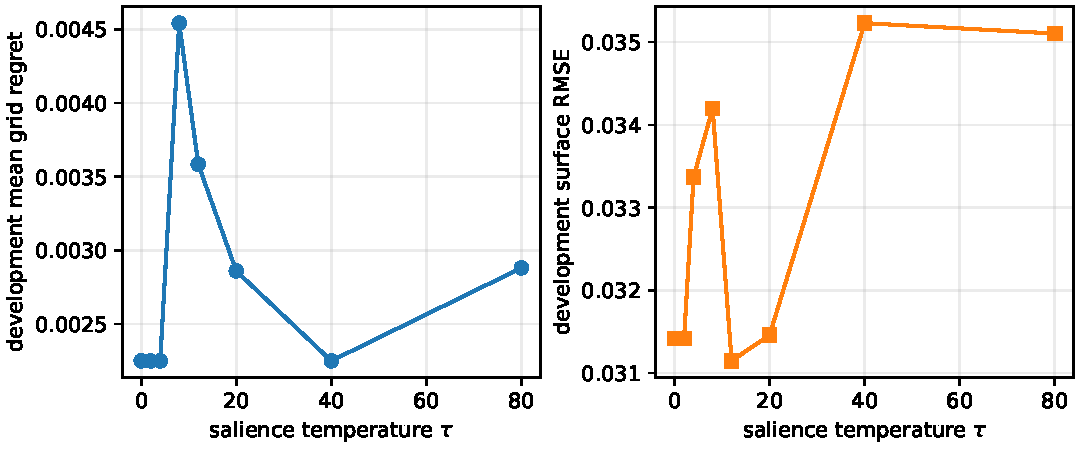
\includegraphics[width=0.72\textwidth]{code/manuscript_assets/figures/temperature_selection.pdf}
\caption{Development-only temperature audit for the gated rule.  Values at
$\tau=0$ and 2 tie within $10^{-12}$, so the frozen rule selects the simpler
uniform weighting $\tau=0$.  The panels report decision and reconstruction
metrics separately.}
\label{fig:temperature}
\end{figure}

\begin{proposition}[Residual reconstruction bounds]
Suppose first that $R_J$ has full column rank.  Then the matrix in
Eq.~\eqref{eq:X} satisfies $X(:,J)=I_r$.  Define
\begin{equation}
\mathcal F_X=\{z\in\RR^N:z=z_JX\}.
\end{equation}
Then $T(f)=f_JX$ interpolates the anchors, is exact for every
$f\in\mathcal F_X$, and obeys
\begin{equation}
\norm{f-T(f)}_\infty
\le (1+\norm{X}_1)
\inf_{z\in\mathcal F_X}\norm{f-z}_\infty.
\label{eq:offsubspace}
\end{equation}
If additionally $\operatorname{rank}(R)=\operatorname{rank}(R_J)=r$, every
row in the training row space belongs to $\mathcal F_X$.

For the gated rule, define the target-dependent restriction distortion
\begin{equation}
\kappa_J(f;R)=\max_i
\frac{\norm{f-R(i,:)}_\infty}{\norm{f_J-R(i,J)}_2},
\label{eq:kappa}
\end{equation}
where a zero-over-zero term is defined as zero and a positive numerator over
zero is $+\infty$.  If
$d_\infty(f,R)=\min_i\norm{f-R(i,:)}_\infty$, then
\begin{equation}
\norm{f-R(i_*(f),:)}_\infty
\le \kappa_J(f;R)\sqrt r\,d_\infty(f,R).
\label{eq:gated-bound}
\end{equation}
Moreover, the gated rule exactly recovers every library row whenever the
anchor restriction distinguishes distinct library rows.
\end{proposition}

\noindent\textit{Proof.}
Because $R_J^\dagger R_J=I_r$,
$X(:,J)=R_J^\dagger R_J=I_r$, and hence
$(T(f))_J=f_J$.  If $f\in\mathcal F_X$, its definition gives $T(f)=f$.
For arbitrary $z\in\mathcal F_X$, linearity and the induced matrix norm give
\begin{align}
\norm{f-T(f)}_\infty
&\le \norm{f-z}_\infty+\norm{T(f-z)}_\infty\\
&\le \norm{f-z}_\infty+\norm{(f-z)_J}_\infty\norm{X}_1\\
&\le(1+\norm{X}_1)\norm{f-z}_\infty.
\end{align}
Taking the infimum proves Eq.~\eqref{eq:offsubspace}.  Under the rank
condition, $\operatorname{col}(R_J)=\operatorname{col}(R)$, so
$R_JR_J^\dagger R=R$.  Therefore
$R=R_JX$ and every linear combination of rows of $R$ is fixed by $T$.
For the gated rule, choose
$k\in\arg\min_i\norm{f-R(i,:)}_\infty$.  The definition of $i_*$ and
Eq.~\eqref{eq:kappa} give
\begin{align}
\norm{f-R(i_*,:)}_\infty
&\le\kappa_J\norm{f_J-R(i_*,J)}_2\\
&\le\kappa_J\norm{f_J-R(k,J)}_2\\
&\le\kappa_J\sqrt r\norm{f-R(k,:)}_\infty,
\end{align}
which is Eq.~\eqref{eq:gated-bound}.  If $f$ is a library row, its anchor
distance is zero; injectivity of the restriction makes every zero-distance
choice the same full row. \hfill$\square$

These are conditional approximation statements.  They neither assert that a
new source residual lies near $\mathcal F_X$ or the library nor control
$\kappa_J$ before the unqueried target residual is known.

\begin{theorem}[Finite-grid decision regret]
For a true response $y\in\RR^N$, a prediction $\widehat y$, and
$\widehat j\in\arg\max_j\widehat y_j$, the regret satisfies
\begin{equation}
0\le \max_j y_j-y_{\widehat j}
\le2\norm{y-\widehat y}_\infty.
\label{eq:regret}
\end{equation}
In particular, if the true best candidate has margin
$\Delta=y_{j_*}-\max_{j\ne j_*}y_j$ and
$\norm{y-\widehat y}_\infty<\Delta/2$, the predicted maximizer is $j_*$.
\end{theorem}

\noindent\textit{Proof.}
Since $\widehat y_{\widehat j}\ge\widehat y_{j_*}$,
\begin{align}
y_{j_*}-y_{\widehat j}
&=(y_{j_*}-\widehat y_{j_*})
+(\widehat y_{j_*}-\widehat y_{\widehat j})
+(\widehat y_{\widehat j}-y_{\widehat j})\\
&\le |y_{j_*}-\widehat y_{j_*}|
+|\widehat y_{\widehat j}-y_{\widehat j}|\\
&\le2\norm{y-\widehat y}_\infty.
\end{align}
If the infinity error is below $\Delta/2$, then for every $j\ne j_*$,
$\widehat y_{j_*}-\widehat y_j>\Delta-2\norm{y-\widehat y}_\infty>0$.
\hfill$\square$

\begin{proposition}[Explicit resource contract]
\label{prop:resources}
For $m\le N$ training tasks and $r\le m$ anchors, standard dense QR with
column pivoting selects the gated anchors in
\begin{equation}
O(Nm^2)\ \text{work},\qquad O(mN)\ \text{storage},
\label{eq:offline}
\end{equation}
in addition to the $mN$ training response evaluations.  For one target,
anchor gating uses exactly $r$ depth-two evaluations, $O(mr+N)$ transfer work,
and $O(mN+N)$ model/workspace storage, plus the analytic depth-one work in
Theorem~1.  Constructing the optional linear map adds
$O(mrN+mr^2)$ work and $O(rN)$ storage; applying it costs $O(rN)$.
Exhaustive search uses $N$ depth-two evaluations.  A nearest-depth-one
transfer uses zero target depth-two evaluations but $O(mN)$ comparison work
and $O(mN)$ stored training data.
\end{proposition}

\noindent\textit{Proof.}
QRCP of an $m$ by $N$ matrix with $m\le N$ costs $O(Nm^2)$.  Gating compares
$m$ restricted rows of length $r$, then copies one length-$N$ row, giving
$O(mr+N)$.  The library contains $mN$ values.  Solving the optional $m$ by
$r$ least-squares problem with $N$ right-hand sides costs
$O(mr^2+mrN)$ and stores $rN$ values.  Obtaining $f_J$ requires exactly the
$r$ selected depth-two responses because its baseline entries are analytic.
The exhaustive and zero-query counts follow by direct enumeration.
\hfill$\square$

Table~\ref{tab:resources} makes these offline and target-time resource counts
comparable under one convention.

\begin{table}[t]
\caption{Work and storage excluding the cost of one depth-two response.
$A\le N$ is the number of distinct first-layer pairs.}
\label{tab:resources}
\begin{ruledtabular}
\scriptsize
\begin{tabular}{@{}lccc@{}}
Method & $p=2$ & Work & Model\\
\hline
Depth-one only & 0 & $O(A|E|+N)$ & $O(N)$\\
Mean residual & 0 & $O(A|E|+N)$ & $O(N)$\\
Nearest $p=1$ & 0 & $O(A|E|+mN)$ & $O(mN)$\\
Anchor-linear & $r$ & $O(A|E|+rN)$ & $O(rN)$\\
Anchor-gated & $r$ & $O(A|E|+mr+N)$ & $O(mN)$\\
Exhaustive & $N$ & $O(N)$ bookkeeping & $O(N)$\\
\end{tabular}
\end{ruledtabular}
\end{table}

\begin{figure}[t]
\centering
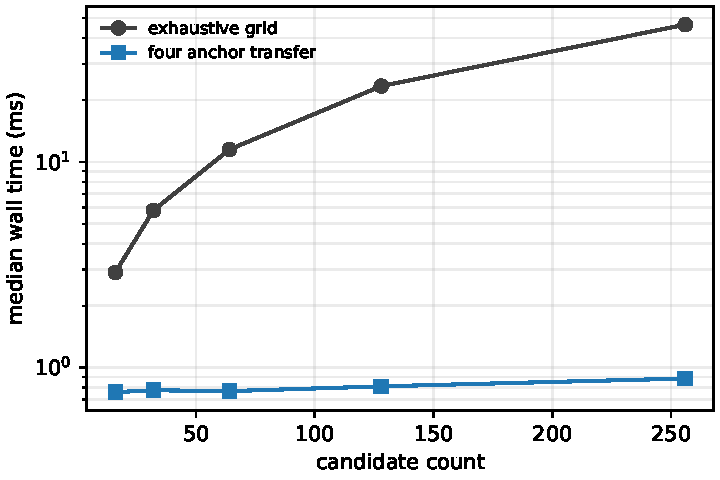
\includegraphics[width=\columnwidth]{code/manuscript_assets/figures/runtime_scaling.pdf}
\caption{Single-host implementation timing on one ten-vertex confirmation
task.  The vertical axis is logarithmic.  These medians illustrate the query
contract; the asymptotic counts are those of
Proposition~\ref{prop:resources}.}
\label{fig:runtime}
\end{figure}

\section{Results: the stronger baseline changes the conclusion}

We report normalized surface RMSE, grid regret, and exact decision fraction.
The comparators are fixed before reading confirmation results:
(i) depth-one only; (ii) the mean training residual; (iii) the residual of the
training task nearest in analytic depth-one-surface RMSE; (iv) uniform-QR
linear reconstruction; (v) QR-anchor-gated residual transfer; (vi) fixed
random anchors; and (vii) uniform-QR reconstruction of the raw surface.

\begin{table}[t]
\caption{Source-disjoint results.  ``Queries'' counts target depth-two
responses.  Development selected $\tau$; confirmation did not select any
method or hyperparameter.  Lower regret/RMSE and higher exact fraction are
better; the confirmation comparison discussed below is read from
Table~\ref{tab:results}.}
\label{tab:results}
\begin{ruledtabular}
\begin{tabular}{lrrrrrrr}
& & \multicolumn{3}{c}{Development: 64 tasks} &
\multicolumn{3}{c}{Confirmation: 16 tasks}\\
Method & Queries & Regret & RMSE & Exact & Regret & RMSE & Exact\\
\hline
Depth-one only & 0 & .068455 & .092466 & .000 & .057170 & .071402 & .000\\
Mean residual & 0 & .008026 & .060075 & .625 & .000000 & .049454 & 1.000\\
Nearest $p=1$ residual & 0 & .002876 & .039463 & .828 & .000000 & .011280 & 1.000\\
Uniform anchor-linear & 4 & .002246 & .033168 & .844 & .000000 & .011811 & 1.000\\
Anchor-gated residual & 4 & .002250 & .031418 & .844 & .000000 & .006095 & 1.000\\
Fixed random anchors & 4 & .103504 & .117963 & .344 & .019824 & .035460 & .625\\
Uniform raw-linear & 4 & .005597 & .038563 & .750 & .000000 & .011821 & 1.000\\
\end{tabular}
\end{ruledtabular}
\end{table}

On development, anchor gating improves the zero-query nearest rule's RMSE by
0.008045 and mean regret by 0.000626, while adding one exact decision out of
64.  Uniform linear interpolation has regret lower by only
$4.1\times10^{-6}$ but RMSE higher by 0.001750.  Figure~\ref{fig:rank} shows
that the ordering is rank-dependent and nonmonotone; more anchors do not
uniformly improve regret.

\begin{figure}[t]
\centering
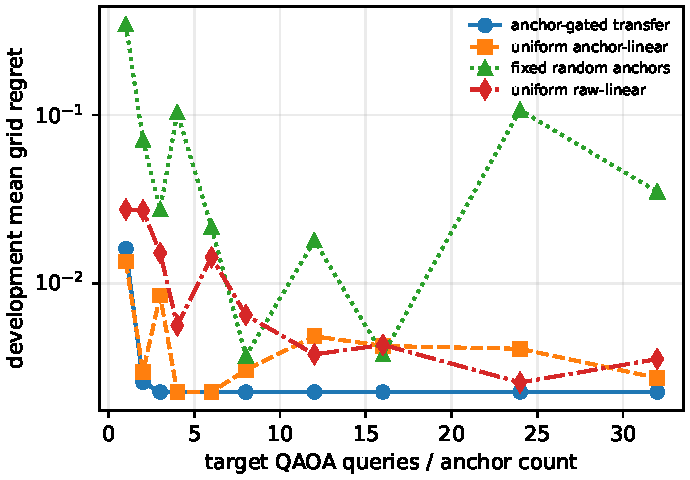
\includegraphics[width=\columnwidth]{code/manuscript_assets/figures/rank_regret.pdf}
\caption{Development mean regret versus target query count.  The registered
primary budget is four.  Nonmonotonic curves preclude a generic ``more rank is
better'' claim.}
\label{fig:rank}
\end{figure}

On confirmation, anchor gating has the smallest nonexhaustive surface RMSE
(Fig.~\ref{fig:rmse}).  Yet the mean-residual and nearest-depth-one rules use
zero depth-two queries and choose the same exact grid maximizer on all 16
tasks; uniform linear and raw-linear rules also score 16/16.  Thus the
confirmation evidence supports better surface reconstruction from the four
anchors, but it cannot attribute correct decisions to those queries.  Because
the confirmation set contains only G67 and G77, $16/16$ is descriptive rather
than a population guarantee.

\begin{figure}[t]
\centering
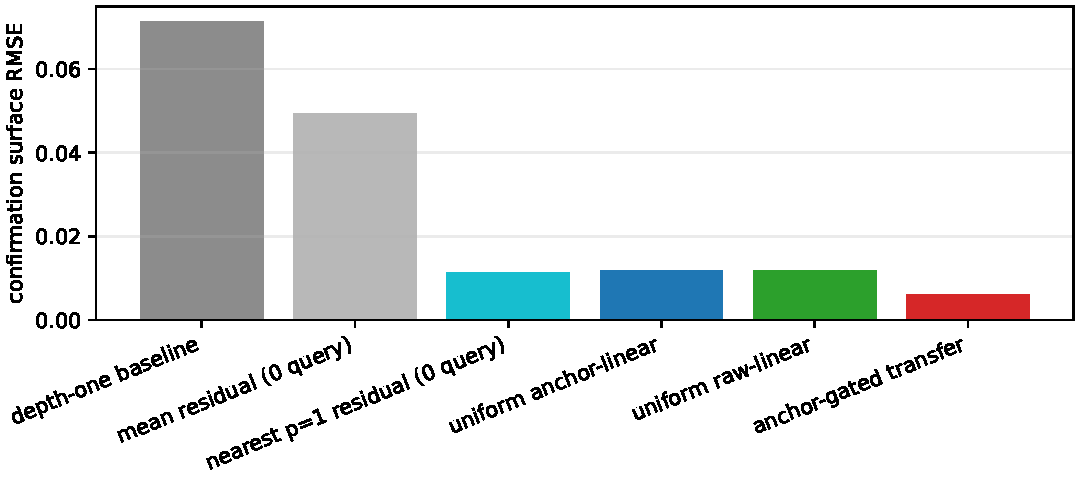
\includegraphics[width=0.78\textwidth]{code/manuscript_assets/figures/confirmation_rmse.pdf}
\caption{Confirmation surface RMSE.  QR-anchor gating is best among the
nonexhaustive comparators.  It and the zero-query nearest-$p=1$ rule
nevertheless make the same 16/16 grid decisions, separating reconstruction
accuracy from evidence of decision-query necessity.}
\label{fig:rmse}
\end{figure}

\section{Measured runtime and its limits}

Figure~\ref{fig:runtime} times the actual Python kernels on one authenticated
G67-derived ten-vertex task under macOS arm64 and Python 3.13.12.  Each point
is the median of seven repetitions after one warm-up.  At $N=256$, exhaustive
state-vector evaluation takes 46.512 ms, while four state-vector evaluations,
analytic baseline construction, and the gated transfer take 0.885 ms.  On
this particular task the transferred surface agrees pointwise with exhaustive
evaluation to $2.22\times10^{-16}$.  This isolated timing is not an
equal-accuracy solver speedup claim across confirmation tasks.  It is also not
a hardware claim: shot noise, compilation, batching, and communication are
absent.

The state vector costs $O(2^{|V|})$ memory and
$O(p|V|2^{|V|}+p|E|2^{|V|})$ arithmetic per response in this implementation.
Nothing here improves that per-query complexity.  Equation~\eqref{eq:predict-gated}
only conditionally substitutes $r$ such responses for $N$ responses after an
offline matrix has been learned.

\section{Reproducibility and claim boundary}

The public package authenticates all 16 source files, recomputes the 128
state-vector landscapes, verifies the locked JSON without overwriting it,
regenerates four figures, and tests the formulas and bounds.  The deterministic
entry point is
\begin{center}
\texttt{qaoa-anchor-reproduce --verify}.
\end{center}
Timing is intentionally separate because wall time is host-specific:
\texttt{qaoa-anchor-benchmark}.  The manifest records hashes and byte counts
for scientific tables, the locked result, timing evidence, and every PDF/PNG
figure.

The following are outside the evidence:
continuous-angle optimization; graph sizes above ten qubits; weighted MaxCut;
noise or quantum hardware; MaxCut approximation ratios or global optima;
statistical independence of tasks from one source; and generalization beyond
the two confirmation sources.  The numerical tests cannot prove the analytic
results; they check implementations and exhibited consequences.  The proofs
above carry the mathematical claims.

\section{Conclusion}

QR-anchor gating is a coherent conditional surrogate: it reduces target
depth-two evaluations from $N$ to $r$, improves development RMSE and regret
over zero-query transfer, and has the smallest confirmation surface RMSE.
But the source-disjoint confirmation data do not show that its four queries
are necessary for the finite-grid decision: two zero-query residual transfers
make every confirmation decision correctly.  The defensible outcome is a
conditional reconstruction result and a sharper next experiment: add many
untouched source families, larger classically tractable graphs, noise-aware
measurements, and predeclared decision baselines before asking whether anchor
queries add out-of-source decision value.

\bibliographystyle{plainnat}
\bibliography{code/manuscript_assets/references}

\end{document}
